% Reviewer 1
\reviewer

\begin{revcomment}
	This paper fails to justify the selection of heuristic factors $(\alpha, \beta)$ in SSF-ACO. You should conduct grid search experiments to demonstrate parameter sensitivity or cite theoretical foundations for ACO parameter tuning.
\end{revcomment}
\begin{revresponse}

\end{revresponse}

\begin{revcomment}
	Current experiments only cover small-scale scenarios ($\leq 30$ nodes), it should extend to more nodes to should the scalibility of algorithm.
\end{revcomment}
\begin{revresponse}
	Thank you for the suggestion.
	Our algorithms are designed with scalability and is capable of handling larger-scale problems.
	To further verify its scalability, we extended the evaluation to include scenarios involving 35 and 40 ground sensor nodes. The updated results are illustrated in Figure~\ref{fig:40nodes}, which is identical to Figure~8a in the manuscript. The results demonstrate that the proposed algorithms continue to exhibit superior performance even in larger-scale scenarios.
	\begin{figure}[h]
		\centerline{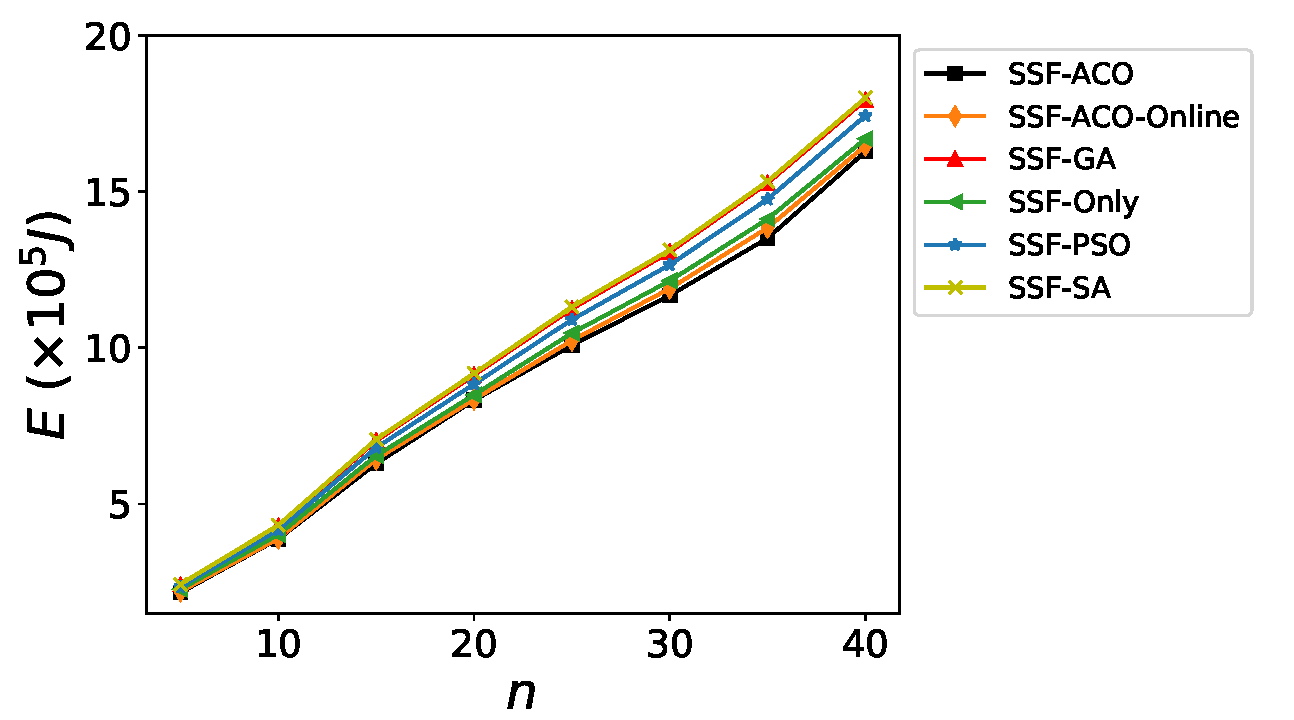
\includegraphics[width=.6\textwidth]{fig/exp_number_40_legend.pdf}}
		\caption{Algorithm performance comparisons in UAV energy consumption under varying numbers of sensors.}
		\label{fig:40nodes}
	\end{figure}
\end{revresponse}

\begin{revcomment}
	The assumptions of linear GN deployment and complete GN knowledge are restrictive and not sufficiently justified. Please provide a detailed discussion of the assumptions, including their implications for real-world applicability and potential extensions.
\end{revcomment}
\begin{revresponse}
	We appreciate the reviewer's comment regarding the assumptions of linear GN deployment and complete GN knowledge.
	We would like to provide additional details about GN deployment and GN knowledge, as well as a discussion of these assumptions in Section 6 of our revised manuscript.

	\textbf{Linear GN deployment.}
	The linear configuration of GNs represents a reasonable and commonly utilized setup in real-world systems.
	This deployment pattern often arises in infrastructure monitoring scenarios.
	For instance, in the power line~\cite{powerline,transmission-line}, UAVs are dispatched to autonomously collect data from sensors on the transmission tower.
	Similarly, in the oil and gas industry~\cite{pipeline}, UAVs are used to fly along pipelines for inspection activities.
	In addition, sensors can be deployed along rivers~\cite{river} and coasts~\cite{coast} to capture diel and seasonal fluctuations, with the purposes of ecological monitoring, flood warning, and scientific research.

	In fact, the effectiveness of such linear GN deployment has already been demonstrated in industrial applications to reduce costs, improve work efficiency, and avoid hazardous manual tasks.
	For instance, DJI has successfully implemented UAV-enabled solutions in scenarios such as long-distance pipelines~\cite{DJI-pipeline}, power transmission line in plateau regions~\cite{DJI-powerline}, and river ecosystems~\cite{DJI-river}, where the UAV trajectories can be regarded as linear or the combination of multiple straight-line segments.

	\textbf{Complete GN knowledge.}
	Sensor knowledge mainly includes information such as position, amount of data to be collected, transmission rate, and data transmission range.
	(1) In the online problem, each sensor has an additional control communication range, which covers a larger area than the data transmission range.
	When the UAV enters the sensor's control communication range, it can detect the sensor and receives a response containing information such as the amount of data and the sensor's position.
	(2) There is a proportional relationship between the radius of the data transmission range and the control communication range.
	Based on the distance between the sensor and the UAV at the moment the response is received, the radius of the data transmission range can be estimated.
	(3) The sensor position is fixed, and thus, it can be obtained during the initial deployment and periodic maintenance. This allows for the calibration of sensor positions.

	\textbf{Discussion in the manuscript.}
	We have extended the discussion of these assumptions in Section 6 of the revised manuscript as follows.
	\begin{changes}
		The UAV keeps broadcasting `Probe' message during the flight to detect sensors. Once receiving the `Probe' message, the sensor sends back an `ACK' message, which includes its position, the amount of data, and transmission characteristics. Note that each sensor sends `ACK' message only once. This partial information availability fundamentally changes the nature of our optimization problem, requiring real-time 
		decision-making based on local information.
	\end{changes}
\end{revresponse}

\begin{revcomment}
	Could the proposed models and algorithms be adapted for 3D GN layouts?
\end{revcomment}
\begin{revresponse}
	Thanks for your comment.
	Our current focuses on the linear (2D) GN distribution, including power transmission lines, roads, pipelines, river and coast. By integrating advanced trajectory planning methods, our algorithms can be extended to 3D GN layout.

	Specifically, we first apply a trajectory planning algorithm to optimize the UAV's flight path and avoid collisions.
	The area of UAV trajectory planning and collision avoidance has been extensively studied in recent years.
	The distance travelled from the starting point to any location along the trajectory is treated as the horizontal coordinate of that location.
	Along this trajectory, we can then use SSF-ACO algorithm to jointly optimize speed and altitude scheduling.
	
	Although promising, this approach to extending the 3D GN layout remains subject to certain limitations.
	Jointly optimizing the 3D trajectory and speed scheduling is expected to have a better performance.
	Furthermore, the increased computational complexity associated with 3D scheduling problems presents additional challenges.
	However, these issue fall within a broader area that extends beyond the focus of the current work.
	Addressing them remains also one of our future research directions.
	In this work we concentrate on the optimization of speed and altitude scheduling, and demonstrate compatibility with existing trajectory planning algorithms.
\end{revresponse}

\begin{revcomment}
	Some statements have inconsistent tenses (e.g. ``Our previous work [20] investigated...''). vs. (``we propose...''), need to unify the full text tense; The reference format should be checked according to IEEE standards (e.g. URL references [6] are not standardized).
\end{revcomment}
\begin{revresponse}
	Thank you for the comment.
	We have carefully reviewed the tense usasge throughout the manuscript and corrected the inconsistent expressions to ensure consistency. Additionally, we have standardized the website reference format according to IEEE Reference Guide.
	% todo 这里要不要把修改的部分复制过来
	% todo 标明是哪几个[xx]
\end{revresponse}

\printpartbibliography{powerline,pipeline,transmission-line,river,coast,DJI-powerline,DJI-pipeline,DJI-river}
